\documentclass[twoside,11pt]{article}

\usepackage{blindtext}
\usepackage{jmlr2e}
\usepackage{amsmath}
\usepackage{booktabs}
\usepackage{multirow}
\usepackage{array}
\usepackage{xcolor}

% Shorthands
\newcommand{\ngx}{\textsc{ngx}}
\newcommand{\spidx}{S\&P~500}
\newcommand{\msciem}{MSCI~EM}
\newcommand{\dataset}{{\cal D}}
\newcommand{\fracpartial}[2]{\frac{\partial #1}{\partial  #2}}

\usepackage{lastpage}
\jmlrheading{319}{2026}{1-\pageref{LastPage}}{}{}{}{Isichei \& Oduwole}
\ShortHeadings{Characterising the Nigerian Stock Exchange for ML-Driven Portfolio Optimisation}{Isichei \& Oduwole}
\firstpageno{1}

\begin{document}
	
	\title{Characterising the Nigerian Stock Exchange
		for Machine Learning-Based Portfolio Research:
		An Empirical Analysis of Return Distributions,
		Volatility Dynamics, Liquidity, and Correlation Structure}
	
	% ==================================================
	% Authors
	% ==================================================
	\author{\name Nnamdi A. Isichei \email augustus@miva.university \\
		\addr Department of Data Science,\\
		School of Computing\\
		Miva Open University, \\
		Abuja, Nigeria
		\AND
		\name Prof. H. K. Oduwole \email oduwolekh@nsuk.edu.ng \\
		\addr Department of Mathematics,\\
		Faculty of Natural \& Applied Sciences\\
		Nasarawa State University,\\
		Keffi, Nigeria}
	
	\editor{}
	\maketitle
	
	% ==================================================
	% Abstract
	% ==================================================
	\begin{abstract}%
		Machine learning portfolio systems encode the statistical assumptions of the markets they were trained on. Deploying such systems on the Nigerian Stock Exchange (\ngx) without first characterising that
		market is methodologically indefensible, yet the \ngx\ is almost entirely absent from the empirical ML-finance literature. This paper fills that gap. Using daily OHLCV data on 22 \ngx\ stocks from
		2015--2025, we document five structural features of the market. All	22 stocks reject normality under the Jarque--Bera test; median excess kurtosis is 4.79 and 19 of 22 stocks are positively skewed. Mean annualised volatility is 43.3\%, with GARCH(1,1) persistence
		$(\alpha + \beta)$ exceeding 0.90 in 12 stocks and a cross-sectional	median of 0.912. The average pairwise return correlation is 0.109, far below typical developed-market levels with a dense
		banking-sector cluster as the only dominant structure. Liquidity risk operates through volume episodicity rather than zero-volume	illiquidity: only 7 zero-volume days occur across the entire dataset, yet the mean volume coefficient of variation is 1.85. At
		the index level, the \ngx\ composite returns a Sharpe ratio of 1.40 over the sample period, nearly double that of the \spidx\ (0.71) at comparable volatility, though nominal Naira figures are materially
		affected by the 2023--2024 devaluation episode. Each finding is translated into a concrete design requirement for the two-stage Graph Neural Network and Reinforcement Learning portfolio framework
		that constitutes the broader research programme of which this characterisation is the empirical foundation.
	\end{abstract}
	
	\begin{keywords}
		Nigerian Stock Exchange, emerging market, microstructure, return distributions, GARCH volatility, liquidity, correlation structure,
		market efficiency, machine learning, portfolio optimisation, African finance
	\end{keywords}
	
	% ========================================================
	\section{Introduction}
	\label{sec:intro}
	
	Classical mean-variance optimisation \citep{markowitz1952portfolio} encodes two assumptions that are particularly fragile in emerging markets: that return distributions are sufficiently normal for
	variance to serve as an adequate risk summary, and that covariance estimates are stable enough to be trusted as inputs to an optimisation routine. In developed markets these assumptions, while imperfect, are workable. In sub-Saharan African markets they routinely fail in ways that are financially consequential \citep{bekaert2023globalized}, and any machine learning model that inherits them will fail in the same direction.
	
	The Nigerian Stock Exchange (\ngx), formally rebranded to NGX Group in 2021, is the largest stock exchange in West Africa and the second-largest in Africa by market capitalisation. It is also almost entirely absent from the ML-finance literature. Published work on ML applications to African markets concentrates overwhelmingly on South African data or treats the continent as a homogeneous frontier \citep{adeabah2023african, naeem2024ml}; Nigeria-specific portfolio research barely exists. This is not merely a gap in coverage, it is a practical problem. A two-stage GNN--RL portfolio system \citep{huang2024, wu2021comprehensive, liang2024portfolio, jiang2024drl}
	designed for the \ngx\ cannot be responsibly built without first knowing what kind of market it is being asked to operate in. The viability of RL-driven approaches in frontier and emerging market contexts has been demonstrated \citep{ngo2023frontier}, and hybrid GNN--RL architectures have shown strong results on major
	exchanges \citep{sun2024graphsage}, but both require careful calibration of market assumptions that the
	present paper provides. Digital infrastructure constraints across Sub-Saharan Africa \citep{kouladoum2022digital} further motivate the need for \ngx-specific empirical grounding before any such system can be responsibly deployed. Distribution shape, volatility persistence, liquidity structure, and correlation architecture are
	not implementation details; they determine which design choices are valid and which will fail out-of-sample.
	
	This paper provides that foundation. It is the empirical answer to Research Question~4 of a broader PhD programme on ML-enhanced portfolio optimisation for the \ngx:
	
	\medskip
	\noindent\textit{What are the unique characteristics of the Nigerian stock market in terms of return distributions, volatility dynamics, liquidity, and correlation structure that require specialised portfolio optimisation approaches?}
	\medskip
	
	We use daily OHLCV data for 22 \ngx\ stocks from 2015--2025, a sample that spans six sectors and covers the COVID-19 shock, the	2023--2024 Naira devaluation, and the subsequent partial recovery. The analysis is five-dimensional distributional properties,	GARCH volatility dynamics, liquidity structure, pairwise
	correlations, and weak-form efficiency, and each finding is connected explicitly to a design requirement for the GNN--RL system under development. To our knowledge, this is the first study to characterise the \ngx\ across all five dimensions simultaneously using a decade of data.
	
	% ========================================================
%	\section{Related Work}
%	\label{sec:related}
%	
%	Return distributions in emerging markets consistently deviate from the normality assumptions that underpin classical portfolio theory. \citet{bekaert2023globalized} document excess kurtosis, time-varying skewness, and regime-dependent volatility across emerging economies, properties that render mean-variance optimisation unreliable as a standalone framework. For Nigeria specifically, \citet{adigwe2015stockmarket} establish strong sensitivity of \ngx\ returns to oil price movements, and \citet{kumeka2022stockafrica} show that Naira-USD exchange rate volatility exerts a material,
%	time-varying influence at the stock level. Neither effect has a close counterpart in currency-stable developed markets, and neither is captured by models calibrated on US or European data.
%	
%	Volatility persistence in frontier and emerging markets is
%	systematically higher than in developed counterparts.
%	GARCH-class models have become the standard tool for capturing conditional heteroscedasticity in this context
%	\citep{bollerslev2023garch}, and \citet{aawaar2023african} report persistence parameters
%	approaching unity for several African equity markets, consistent with slow mean-reversion of conditional variance. This matters for portfolio construction: a volatility estimate that decays quickly after a shock, the developed-market norm will systematically
%	understate risk in the periods immediately following a
%	high-volatility episode. On liquidity, the conventional view that zero-volume days constitute the primary constraint for African institutional investors \citep{bekaert2007liquidity} has been challenged by \citet{ngene2022volume}, who show that the operative
%	risk is extreme volume variability rather than outright absence of trading, a distinction with direct implications for any strategy requiring regular rebalancing.
%	
%	Correlation structure and market efficiency complete the picture. \citet{bekaert2023globalized} show that within-market correlations in emerging economies remain structurally different from developed markets, while \citet{emenike2021westafrica} find evidence of low cross-stock correlations within West African markets, consistent with segmentation from global factors and suggesting within-country diversification opportunities that standard developed-market models would not predict. Weak-form efficiency tests on African markets yield mixed results: price series are generally consistent with a
%	random walk in levels, but detectable short-horizon autocorrelations in daily returns have been reported \citep{ferrouhi2021calendar}, leaving open the possibility that pattern-based ML models can extract predictive signal that classical technical analysis cannot.
	\section{Related Work}
	\label{sec:related}
	
	Return distributions in emerging markets deviate consistently from the normality assumptions underlying classical portfolio theory. \citet{bekaert2023globalized} document excess kurtosis, time-varying skewness, and regime-dependent volatility across emerging economies, rendering mean-variance optimisation unreliable as a standalone framework. For Nigeria, \citet{adigwe2015stockmarket} show strong sensitivity of \ngx\ returns to oil prices, while \citet{kumeka2022stockafrica} find that Naira-USD exchange rate volatility exerts a material, time-varying influence at the stock level. Neither effect has a close counterpart in currency-stable developed markets nor is captured by models calibrated on US or European data.
	
	Volatility persistence in frontier and emerging markets is systematically higher than in developed counterparts. GARCH-class models remain the standard for capturing conditional heteroscedasticity \citep{bollerslev2023garch}, and \citet{aawaar2023african} report persistence parameters approaching unity in several African markets, consistent with slow mean reversion of conditional variance. This has direct portfolio implications: estimates that decay quickly after shocks, the developed-market norm will understate post-shock risk. On liquidity, the view that zero-volume days are the primary constraint \citep{bekaert2007liquidity} is challenged by \citet{ngene2022volume}, who show that extreme volume variability, rather than trading absence, is the operative risk, with implications for strategies requiring regular rebalancing.
	
	Correlation structure and market efficiency complete the picture. \citet{bekaert2023globalized} show that within-market correlations in emerging economies differ structurally from developed markets, while \citet{emenike2021westafrica} find low cross-stock correlations in West Africa, consistent with segmentation from global factors and implying diversification opportunities not predicted by standard models. Weak-form efficiency evidence is mixed: price series broadly follow a random walk in levels, but short-horizon autocorrelations in daily returns persist \citep{ferrouhi2021calendar}, leaving scope for ML models to extract predictive signal beyond classical technical analysis.
	
	% ========================================================
%	\section{Data and Methodology}
%	\label{sec:data}
%	
%	\subsection{Dataset}
%	
%	The dataset comprises daily OHLCV data for 22 \ngx\ equities from 2 January 2015 to 31 December 2025, yielding approximately 2,520 trading days per stock across six sectors. Data were sourced from the NGX official portal and cross-validated against Investing.com.
%	All prices are adjusted for corporate actions. Gaps of three or fewer days were filled by linear interpolation; stocks below 95\% completeness were excluded. Table~\ref{tab:universe} reports the full universe.
%	
%	Selecting the most liquid and data-complete stocks introduces liquidity and survivorship bias: the universe overrepresents operationally stable companies and will not fully reflect the statistical properties of the broader NGX listing. This is a deliberate choice. The research objective is to characterise the \emph{investable} universe available to a Nigerian institutional investor, not the entire listed market, and the findings should be interpreted accordingly.
%	
%	Linear interpolation is not without risk in thin markets, where a missing observation signals the absence of price discovery rather than a data error, and smoothing it away can dampen measured volatility and distort GARCH persistence estimates. In practice the exposure here is negligible: only seven zero-volume observations	exist across the entire dataset, two for PRESCO, five for SEPLAT,	with no gap longer than a single day affecting at most 0.002\%	of the observations used in estimation.
	\section{Data and Methodology}
	\label{sec:data}
	
	\subsection{Dataset}
	
	The dataset comprises daily OHLCV data for 22 \ngx\ equities from 2 January 2015 to 31 December 2025, yielding approximately 2,520 trading days per stock across six sectors. Data were sourced from the NGX official portal and cross-validated against Investing.com. All prices are adjusted for corporate actions. Gaps of three or fewer days were filled by linear interpolation; stocks below 95\% completeness were excluded. Table~\ref{tab:universe} reports the full universe.
	
	Selecting the most liquid and data-complete stocks introduces liquidity and survivorship bias: the universe overrepresents operationally stable firms and does not fully capture the statistical properties of the broader NGX listing. This is intentional. The objective is to characterise the \emph{investable} universe available to a Nigerian institutional investor, not the entire market, and findings should be interpreted accordingly.
	
	Linear interpolation is not without risk in thin markets, where missing observations may reflect absent price discovery rather than data error; smoothing can dampen measured volatility and distort GARCH persistence. In practice, the exposure is negligible: only seven zero-volume observations exist two for PRESCO and five for SEPLAT with no gap longer than one day, affecting at most 0.002\% of observations used in estimation.
	
	\begin{table}[ht]
		\centering
		\caption{The 22-stock \ngx\ research universe. Ann.\ return
			$= \bar{r} \times 252$; Ann.\ vol $= \hat{\sigma}\sqrt{252}$;
			computed from daily log returns. TRANSCO and UCAP are extreme
			outliers discussed in Section~\ref{sec:dist}.}
		\label{tab:universe}
		\small
		\setlength{\tabcolsep}{5pt}
		\begin{tabular}{llrrrr}
			\toprule
			\textbf{Ticker} & \textbf{Sector} &
			\textbf{Ret (\%)} & \textbf{Vol (\%)} &
			\textbf{Skew} & \textbf{Kurt}\\
			\midrule
			DANGCEM   & Industrials     & 16.3 & 33.1 &  0.20 &  9.78 \\
			DANGSUG   & Consumer Goods  & 32.1 & 46.7 &  0.34 &  3.45 \\
			ETI       & Financial Svcs  & 18.9 & 46.1 &  0.08 &  3.35 \\
			FCMB      & Financial Svcs  & 27.5 & 51.0 &  0.32 &  1.62 \\
			FIDELIT   & Financial Svcs  & 34.7 & 48.7 &  0.14 &  2.86 \\
			FIRSTHOLD & Financial Svcs  & 27.6 & 48.8 &  0.41 &  2.55 \\
			GTCO      & Financial Svcs  & 18.8 & 37.2 &  0.05 &  4.79 \\
			GUINNES   & Consumer Goods  & 16.3 & 43.4 &  0.31 &  5.25 \\
			IBTC      & Financial Svcs  & 19.5 & 39.1 &  0.11 &  5.81 \\
			INTBREW   & Consumer Goods  &  9.9 & 53.5 &  0.26 &  2.24 \\
			NB        & Consumer Goods  &  3.4 & 41.3 &  0.29 &  4.62 \\
			NESTLE    & Consumer Goods  & 11.1 & 31.1 &  0.55 & 11.41 \\
			OKOMUOI   & Agriculture     & 42.6 & 39.1 &  0.74 &  6.90 \\
			PRESCO    & Agriculture     & 45.8 & 38.9 &  0.57 &  5.98 \\
			SEPLAT    & Oil \& Gas      & 32.7 & 35.8 &  0.71 & 10.26 \\
			STERLINGNG& Financial Svcs  & 22.5 & 50.3 &  0.24 &  1.91 \\
			TOTAL     & Oil \& Gas      & 19.5 & 34.7 &  0.53 &  8.44 \\
			TRANSCO$^\dagger$ & Conglomerate & 78.8 & 150.6 & 28.2 & 968.4\\
			UBA       & Financial Svcs  & 30.6 & 43.9 & -0.01 &  4.53 \\
			UCAP$^\dagger$    & Financial Svcs  & 38.3 & 52.6 & -3.27 & 64.4\\
			WAPCO     & Industrials     & 20.4 & 54.5 &  0.12 &  3.10 \\
			ZENITHB   & Financial Svcs  & 19.1 & 39.0 & -0.28 &  7.30 \\
			\midrule
			\textit{Mean (excl.\ $^\dagger$)} & &
			\textit{24.2} & \textit{43.3} &
			\textit{0.25} & \textit{5.25}\\
			\bottomrule
			\multicolumn{6}{l}{$^\dagger$ Extreme outlier; treated separately throughout.}
		\end{tabular}
	\end{table}
	
	\subsection{Analytical Methods}
	
	Five analytical layers are applied. \textbf{Return distributions:}	daily log returns $r_t = \ln(P_t/P_{t-1})$; skewness, excess	kurtosis, and the Jarque--Bera statistic
	\begin{equation}
		\mathrm{JB} = \frac{n}{6}\!\left(S^2 + \frac{(K-3)^2}{4}\right)
		\sim \chi^2(2)
		\label{eq:jb}
	\end{equation}
	where $S$ is sample skewness and $K$ is sample kurtosis; and 1-day 95\% VaR and CVaR under historical simulation. \textbf{Volatility dynamics:} GARCH(1,1) estimated for each stock,
	\begin{equation}
		\sigma_t^2 = \omega + \alpha\varepsilon_{t-1}^2
		+ \beta\sigma_{t-1}^2
		\label{eq:garch}
	\end{equation}
	with $\alpha + \beta$ as the persistence summary. A uniform specification is used across all 22 stocks to keep persistence estimates directly comparable and to avoid the data-mining risk inherent in searching each series for its preferred model. The	leverage-effect literature formalised by \citet{nelson1991egarch}
	and \citet{glosten1993gjr} and applied specifically to the \ngx\ by \citet{adams2024asymmetric}, raises a legitimate case for	asymmetric specifications such as EGARCH and GJR-GARCH; we treat that as a direction for the full model development phase rather than a deficiency of the present cross-sectional analysis. \textbf{Liquidity:} We measure (i) the zero-volume rate and	(ii) the coefficient of variation of daily volume,
	$\mathrm{CV}_i = \sigma_{\mathrm{vol},i}/\mu_{\mathrm{vol},i}$, which captures episodic trading activity.
	\textbf{Correlation structure:} the full $22\times22$ Pearson	correlation matrix of daily log returns; distributional statistics across all 231 unique off-diagonal pairs. \textbf{Market efficiency:}
	Augmented Dickey--Fuller tests on price levels; lag-1 return autocorrelation for serial dependence.
	
	% =======================================================
%	\section{Return Distribution Analysis}
%	\label{sec:dist}
%	
%	The Jarque--Bera test rejects normality for all 22 stocks: 18 yield $p \approx 0$ to machine precision; the remaining four (FCMB, FIDELIT, FIRSTHOLD, INTBREW) yield $p < 10^{-74}$. Excluding TRANSCO, the cross-sectional median excess kurtosis is 4.79, with ten stocks exceeding 5.0.
%	
%	Two stocks require separate treatment throughout the analysis. TRANSCO carries kurtosis of 968.4 and skewness of 28.25, statistics consistent with a handful of catastrophic price moves that no standard distribution can accommodate and its GARCH persistence equals exactly 1.000, indicating a unit root in the variance process. UCAP records kurtosis of 64.4 and skewness of $-3.27$, strongly negative in a universe where 19 of 22 stocks lean
%	right; its persistence of 0.378, the lowest in the universe by	a wide margin points to isolated price dislocations rather than structural volatility clustering. Both would be excluded from the	investable universe by the statistical screening filters of the
%	broader ML pipeline.
%	
%	Among the remaining 20 stocks, 19 exhibit positive skewness. This is the opposite of what one observes in developed markets, where negative skewness reflecting crash risk is the norm, and it contrasts with both the \spidx\ and \msciem, which are negatively skewed over the same period (Table~\ref{tab:comparison}). The most
%	pronounced right-tail asymmetry appears in OKOMUOI (0.74), SEPLAT (0.71), and PRESCO (0.57). The practical consequence for the RL portfolio agent is direct: symmetric, variance-based loss functions are mis-specified for this universe. Reward functions must penalise CVaR and maximum drawdown rather than variance, which treats upside	and downside deviations identically.
%	
%	Table~\ref{tab:risk} reports 1-day 95\% VaR and CVaR for all stocks.	The CVaR--VaR spread exceeds 200 basis points universally; the	widest gaps; UCAP (316 bps), INTBREW (283 bps), WAPCO (250 bps), signal distributions where a genuinely bad day is substantially worse than the 5th-percentile threshold alone would suggest. Any
%	risk model that stops at VaR will systematically understate tail	exposure in \ngx\ equities.
%	
%	\begin{table}[ht]
%		\centering
%		\caption{1-day 95\% VaR and CVaR under historical simulation.
%			The CVaR--VaR spread measures severity of losses beyond the
%			VaR threshold.}
%		\label{tab:risk}
%		\small
%		\begin{tabular}{lrr|lrr}
%			\toprule
%			\textbf{Stock} & \textbf{VaR} & \textbf{CVaR} &
%			\textbf{Stock} & \textbf{VaR} & \textbf{CVaR}\\
%			\midrule
%			NESTLE    & $-2.7$\% & $-5.0$\% & SEPLAT    & $-2.7$\% & $-5.8$\%\\
%			DANGCEM   & $-2.9$\% & $-5.5$\% & TOTAL     & $-3.7$\% & $-5.5$\%\\
%			GTCO      & $-3.4$\% & $-5.6$\% & ZENITHB   & $-3.5$\% & $-5.8$\%\\
%			OKOMUOI   & $-4.0$\% & $-5.9$\% & IBTC      & $-4.0$\% & $-6.2$\%\\
%			PRESCO    & $-3.8$\% & $-5.8$\% & UBA       & $-4.2$\% & $-6.4$\%\\
%			DANGSUG   & $-4.7$\% & $-6.8$\% & NB        & $-4.3$\% & $-6.4$\%\\
%			ETI       & $-4.8$\% & $-7.2$\% & STERLINGNG& $-4.7$\% & $-7.0$\%\\
%			FIDELIT   & $-4.7$\% & $-6.6$\% & FCMB      & $-4.9$\% & $-6.9$\%\\
%			FIRSTHOLD & $-4.8$\% & $-6.8$\% & UCAP      & $-4.4$\% & $-7.6$\%\\
%			GUINNES   & $-4.6$\% & $-6.9$\% & INTBREW   & $-5.1$\% & $-7.9$\%\\
%			WAPCO     & $-6.1$\% & $-8.6$\% & TRANSCO   & $-5.3$\% & $-8.2$\%\\
%			\bottomrule
%		\end{tabular}
%	\end{table}
	
	\section{Return Distribution Analysis}
	\label{sec:dist}
	
	The Jarque--Bera test rejects normality for all 22 stocks: 18 yield $p \approx 0$ to machine precision, while the remaining four (FCMB, FIDELIT, FIRSTHOLD, INTBREW) have $p < 10^{-74}$. Excluding TRANSCO, the cross-sectional median excess kurtosis is 4.79, with ten stocks above 5.0.
	
	Two stocks require separate treatment. TRANSCO shows kurtosis of 968.4 and skewness of 28.25, consistent with a few catastrophic price moves beyond standard distributions; its GARCH persistence equals 1.000, indicating a unit root in variance. UCAP records kurtosis of 64.4 and skewness of $-3.27$, strongly negative in a universe where 19 of 22 stocks lean right. Its persistence of 0.378, the lowest by a wide margin, suggests isolated price dislocations rather than structural volatility clustering. Both would be excluded from the investable universe by ML screening filters.
	
	Among the remaining 20 stocks, 19 exhibit positive skewness, opposite to developed markets where negative skewness dominates and in contrast to both the \spidx\ and \msciem (Table~\ref{tab:comparison}). The strongest right-tail asymmetry appears in OKOMUOI (0.74), SEPLAT (0.71), and PRESCO (0.57). For the RL portfolio agent, symmetric variance-based loss functions are therefore mis-specified; reward functions should penalise CVaR and maximum drawdown rather than variance.
	
	Table~\ref{tab:risk} reports 1-day 95\% VaR and CVaR. The CVaR--VaR spread exceeds 200 bps across all stocks; the widest gaps; UCAP (316 bps), INTBREW (283 bps), and WAPCO (250 bps), indicate that realised losses can far exceed the 5th-percentile threshold. Models relying only on VaR will understate tail risk in \ngx\ equities.
	
	\begin{table}[ht]
		\centering
		\caption{1-day 95\% VaR and CVaR under historical simulation.
			The CVaR--VaR spread measures severity of losses beyond the
			VaR threshold.}
		\label{tab:risk}
		\small
		\begin{tabular}{lrr|lrr|lrr}
			\toprule
			\textbf{Stock} & \textbf{VaR} & \textbf{CVaR} &
			\textbf{Stock} & \textbf{VaR} & \textbf{CVaR} &
			\textbf{Stock} & \textbf{VaR} & \textbf{CVaR} \\
			\midrule
			NESTLE    & $-2.7$\% & $-5.0$\% & ETI        & $-4.8$\% & $-7.2$\% & NB         & $-4.3$\% & $-6.4$\% \\
			DANGCEM   & $-2.9$\% & $-5.5$\% & FIDELIT    & $-4.7$\% & $-6.6$\% & STERLINGNG & $-4.7$\% & $-7.0$\% \\
			GTCO      & $-3.4$\% & $-5.6$\% & FIRSTHOLD  & $-4.8$\% & $-6.8$\% & FCMB       & $-4.9$\% & $-6.9$\% \\
			OKOMUOI   & $-4.0$\% & $-5.9$\% & GUINNES    & $-4.6$\% & $-6.9$\% & UCAP       & $-4.4$\% & $-7.6$\% \\
			PRESCO    & $-3.8$\% & $-5.8$\% & WAPCO      & $-6.1$\% & $-8.6$\% & INTBREW    & $-5.1$\% & $-7.9$\% \\
			DANGSUG   & $-4.7$\% & $-6.8$\% & SEPLAT     & $-2.7$\% & $-5.8$\% & TRANSCO    & $-5.3$\% & $-8.2$\% \\
			ETI       & $-4.8$\% & $-7.2$\% & TOTAL      & $-3.7$\% & $-5.5$\% &            &          &           \\
			FIDELIT   & $-4.7$\% & $-6.6$\% & ZENITHB    & $-3.5$\% & $-5.8$\% &            &          &           \\
			\bottomrule
		\end{tabular}
	\end{table}
	% ============================================================
%	\section{Volatility Dynamics}
%	\label{sec:vol}
%	
%	Excluding TRANSCO (annualised vol 150.6\%), mean annualised
%	volatility across the universe is 43.3\%, ranging from 31.1\%
%	(NESTLE) to 54.5\% (WAPCO). The \ngx\ composite records 19.0\%
%	over the same period --- roughly half the individual stock average
%	--- confirming that substantial idiosyncratic risk partially
%	diversifies away at the index level. Figure~\ref{fig:vol_clustering}
%	illustrates the clustering property directly, contrasting six stocks
%	chosen to span the persistence spectrum across the five major event
%	windows of the sample period.
%	
%	Table~\ref{tab:garch} reports the GARCH(1,1) estimates.
%	\citet{engle2023covol} show that major macro shocks transmit
%	volatility internationally, a channel that bears directly on an
%	oil-dependent economy where global commodity prices are a known
%	amplifier of domestic equity risk. Three findings emerge from the
%	estimates. First, 12 of 22 stocks exhibit $\alpha + \beta > 0.90$
%	--- DANGSUG, ETI, FIDELIT, FIRSTHOLD, GTCO, NB, STERLINGNG,
%	TOTAL, TRANSCO, UBA, WAPCO, and ZENITHB --- with FIRSTHOLD
%	reaching 0.947, implying a volatility shock half-life exceeding 12
%	trading days. Second, the cross-sectional median persistence of
%	0.912 (excluding TRANSCO and UCAP) clearly exceeds the 0.80--0.85
%	range reported for US individual stocks in the literature
%	\citep{aawaar2023african, bollerslev2023garch}; the mean of 0.836
%	sits at the upper bound of that range. The distribution of
%	persistence parameters across the \ngx\ is shifted materially
%	upward relative to developed markets --- volatility here is both
%	higher in level and slower to mean-revert. Third, UCAP's persistence
%	of 0.378 is the lowest in the universe and, combined with its
%	kurtosis of 64.4, points to isolated price dislocations rather than
%	sustained clustering, distinguishing it sharply from TRANSCO whose
%	unit-root variance process implies ongoing structural instability.
%	Static covariance matrices will therefore be biased during and after
%	high-volatility regimes; the RL agent's state vector must include
%	time-varying volatility features --- rolling realised variance and
%	GARCH-implied conditional variance --- to enable dynamic
%	position-sizing as market conditions evolve.
%	
%	\begin{figure}[ht]
%		\centering
%		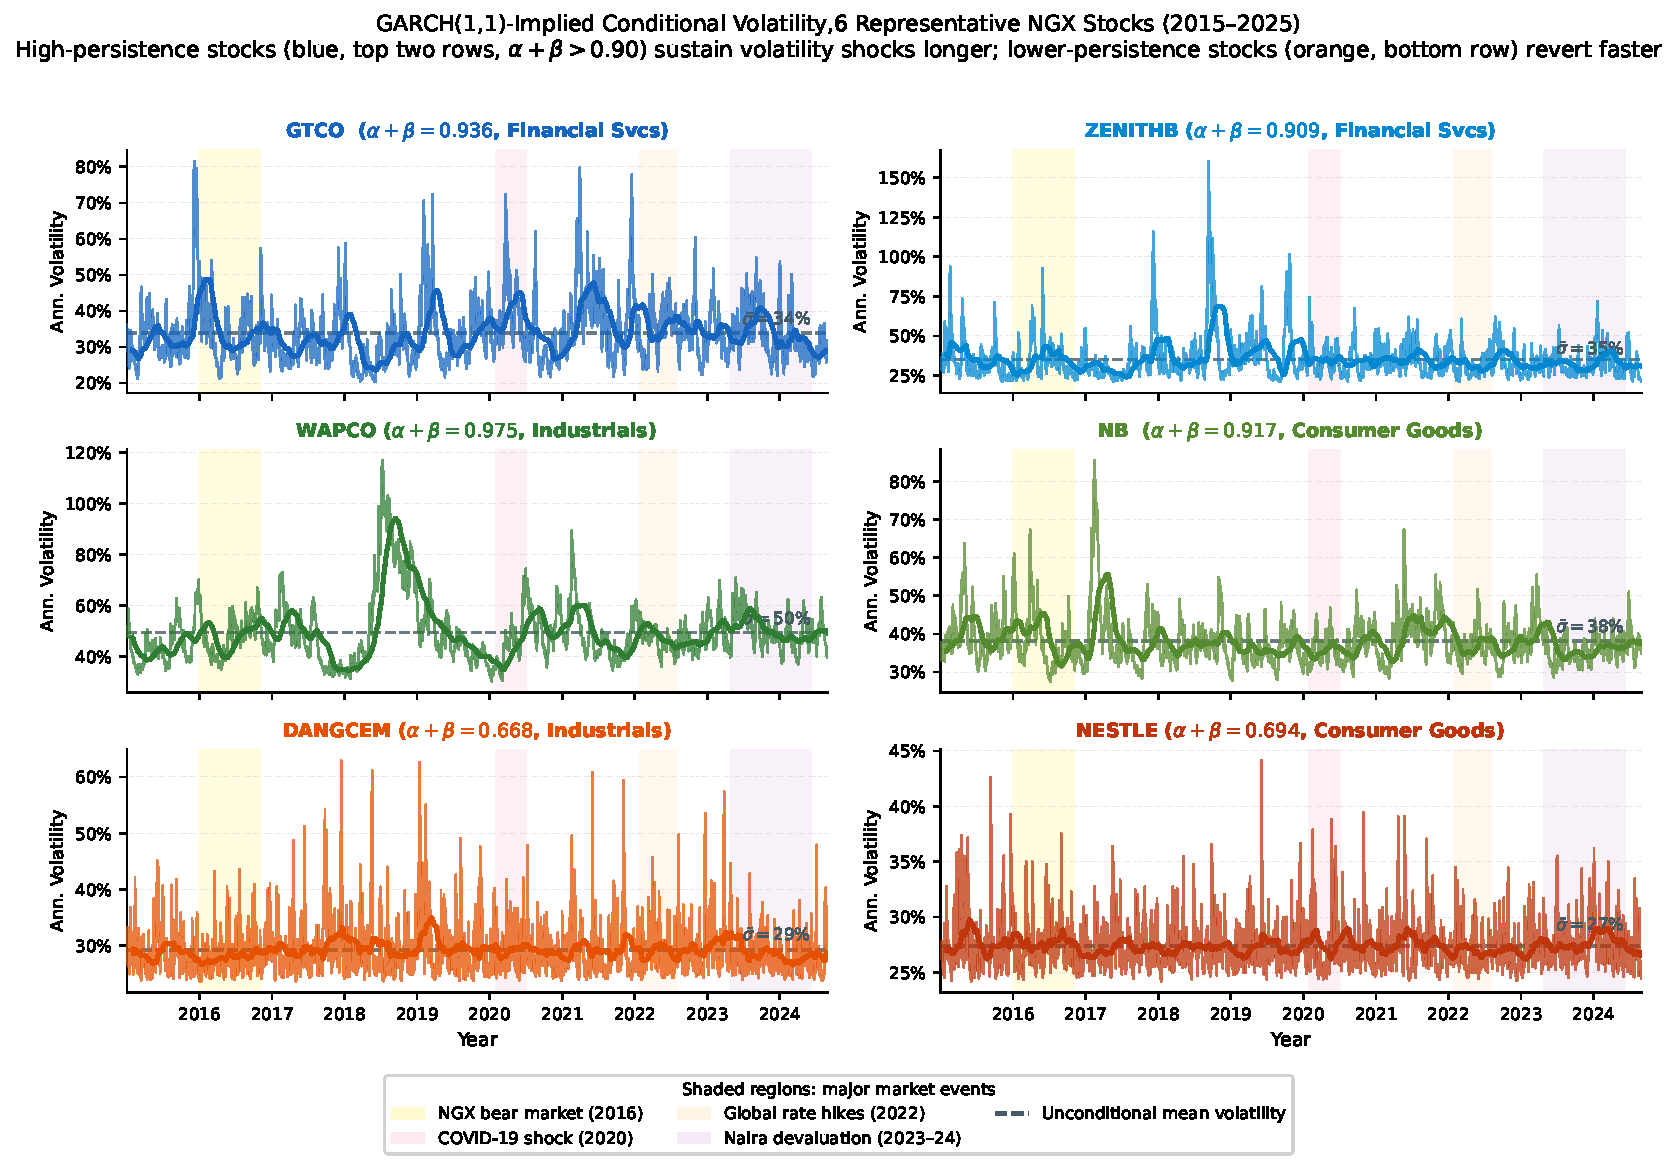
\includegraphics[width=\linewidth]{fig2_volatility_clustering.pdf}
%		\caption{GARCH(1,1)-implied conditional annualised volatility for
%			six representative \ngx\ stocks (2015--2025), contrasting
%			high-persistence ($\alpha + \beta > 0.90$, top two rows)
%			against lower-persistence ($\alpha + \beta < 0.70$, bottom
%			row) dynamics. Thick lines show the 63-day rolling mean;
%			thin lines the daily series; dashed horizontals the
%			unconditional mean. Shaded regions mark the 2016 \ngx\ bear
%			market, the 2020 COVID-19 shock, the 2022 global rate hiking
%			cycle, and the 2023--2024 Naira devaluation.}
%		\label{fig:vol_clustering}
%	\end{figure}
%	

	\section{Volatility Dynamics}
	\label{sec:vol}
	
	Excluding TRANSCO (annualised vol 150.6\%), mean annualised volatility across the universe is 43.3\%, ranging from 31.1\% (NESTLE) to 54.5\% (WAPCO). The \ngx\ composite records 19.0\% over the same period, roughly half the individual stock average confirming that substantial idiosyncratic risk partially diversifies at the index level. Figure~\ref{fig:vol_clustering} illustrates volatility clustering for six stocks spanning the persistence spectrum across five major event windows.
	
	Table~\ref{tab:garch} reports GARCH(1,1) estimates. \citet{engle2023covol} show that major macro shocks transmit volatility internationally, a channel relevant for an oil-dependent economy where global commodity prices amplify domestic equity risk. Three findings emerge. First, 12 of 22 stocks exhibit $\alpha + \beta > 0.90$, DANGSUG, ETI, FIDELIT, FIRSTHOLD, GTCO, NB, STERLINGNG, TOTAL, TRANSCO, UBA, WAPCO, and ZENITHB, with FIRSTHOLD reaching 0.947, implying a volatility shock half-life exceeding 12 trading days. Second, the median persistence of 0.912 (excluding TRANSCO and UCAP) exceeds the 0.80--0.85 range reported for US stocks \citep{aawaar2023african, bollerslev2023garch}; the mean of 0.836 lies at the upper bound. Persistence in the \ngx\ is thus materially higher volatility is both elevated and slower to mean-revert. Third, UCAP’s persistence of 0.378, alongside kurtosis of 64.4, indicates isolated price dislocations rather than sustained clustering, in contrast to TRANSCO’s unit-root variance process implying structural instability. Static covariance matrices will therefore be biased during and after high-volatility regimes; the RL agent’s state vector should include time-varying volatility features rolling realised variance and GARCH-implied conditional variance to support dynamic position sizing.
	
	\begin{figure}[ht]
		\centering
		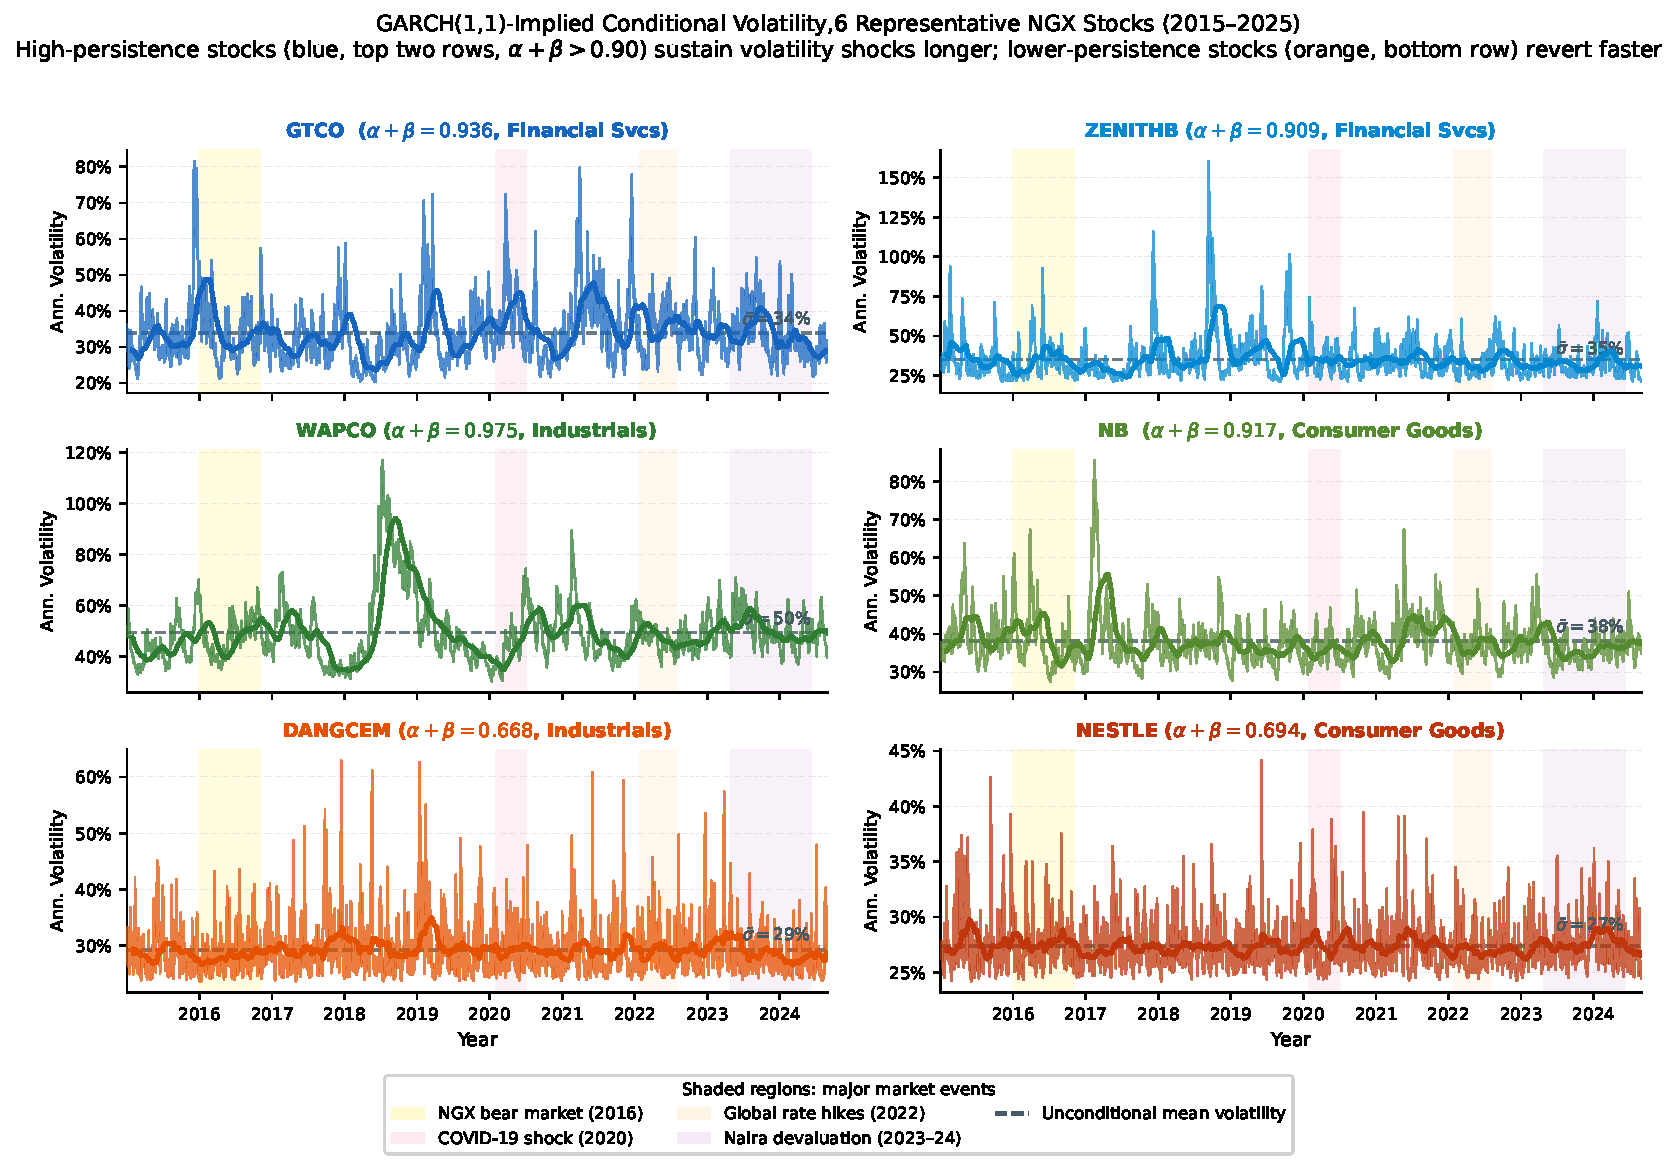
\includegraphics[width=\linewidth]{fig2_volatility_clustering.pdf}
		\vspace{-30pt}
		\label{fig:vol_clustering}
	\end{figure}
	\begin{figure}
		\caption{GARCH(1,1) conditional annualised volatility for six \ngx\ stocks (2015--2025), contrasting high ($\alpha+\beta>0.90$) and low ($\alpha+\beta<0.70$) persistence. Thick lines show 63-day means, thin lines daily series, dashed lines unconditional means; shaded regions denote major market events.}
		\vspace{-20pt}
	\end{figure}
	\begin{table}[ht]
		\centering
		\small
		\setlength{\belowcaptionskip}{5pt} 
		\caption{GARCH(1,1) parameter estimates. $\alpha + \beta$ values in \textbf{bold} exceed 0.90.}
		\label{tab:garch}
		\setlength{\tabcolsep}{4pt} 
		\begin{tabular}{lcccc | lcccc}
			\toprule
			\textbf{Stock} & $\omega\times10^4$ & $\alpha$ & $\beta$ & $\alpha+\beta$ & \textbf{Stock} & $\omega\times10^4$ & $\alpha$ & $\beta$ & $\alpha+\beta$ \\
			\midrule
			DANGCEM    & 14.82 & 0.197 & 0.471 & 0.668          & NESTLE     & 11.87 & 0.098 & 0.595 & 0.694 \\
			DANGSUG    & 5.82  & 0.106 & 0.827 & \textbf{0.932} & OKOMUOI    & 13.37 & 0.180 & 0.616 & 0.796 \\
			ETI        & 6.80  & 0.099 & 0.818 & \textbf{0.917} & PRESCO     & 15.34 & 0.190 & 0.573 & 0.763 \\
			FCMB       & 13.62 & 0.220 & 0.659 & 0.879          & SEPLAT     & 14.43 & 0.107 & 0.608 & 0.715 \\
			FIDELIT    & 7.09  & 0.175 & 0.761 & \textbf{0.935} & STERLINGNG & 8.25  & 0.182 & 0.736 & \textbf{0.918} \\
			FIRSTHOLD  & 6.08  & 0.200 & 0.746 & \textbf{0.947} & TOTAL      & 4.46  & 0.122 & 0.793 & \textbf{0.915} \\
			GTCO       & 4.02  & 0.169 & 0.767 & \textbf{0.936} & TRANSCO$^\dagger$ & 53.39 & 0.111 & 0.889 & \textbf{1.000} \\
			GUINNES    & 11.10 & 0.138 & 0.716 & 0.854          & UBA        & 7.40  & 0.244 & 0.684 & \textbf{0.928} \\
			IBTC       & 11.14 & 0.106 & 0.711 & 0.817          & UCAP       & 71.15 & 0.197 & 0.181 & 0.378 \\
			INTBREW    & 27.50 & 0.151 & 0.604 & 0.755          & WAPCO      & 2.73  & 0.078 & 0.897 & \textbf{0.975} \\
			NB         & 5.60  & 0.091 & 0.826 & \textbf{0.917} & ZENITHB    & 6.30  & 0.221 & 0.688 & \textbf{0.909} \\
			\midrule
			\multicolumn{10}{l}{\textit{Mean (excl.\ $^\dagger$)}: \textit{0.836}} \\
			\bottomrule
			\multicolumn{10}{l}{$^\dagger$ Unit root in variance; see text.}
		\end{tabular}
	\end{table}
	
	% ============================================================
	\section{Liquidity Structure}
	\label{sec:liquidity}
	
	The received assumption that zero-trading days constitute the binding	liquidity constraint for African equity portfolios does not hold for this universe. Only seven zero-volume days occur across all 22 stocks over the full decade, two for PRESCO (0.074\%) and five for SEPLAT
	(0.186\%) with every other stock recording positive volume on every available trading day. The operative risk is not absence of trading but its irregularity.
	
	\emph{Volume episodicity} infrequent bursts of institutional-scale	activity interspersed with extended low-turnover periods is	captured jointly by the coefficient of variation (CV) and the median-to-mean volume ratio. A high CV signals an irregular volume
	distribution; a median-to-mean ratio far below unity confirms that the mean is pulled upward by the minority of high-activity sessions rather than reflecting a typical trading day. Table~\ref{tab:liquidity}
	documents both metrics across the universe.
	
	The cross-sectional mean CV of 1.85 indicates that the volume standard deviation exceeds the mean by a factor approaching two. Three stocks; UCAP (CV 3.55), TRANSCO (3.45), FIDELIT (3.43),	are so dominated by episodic activity that the mean volume figure is practically uninformative. NB and DANGSUG are the starkest cases on
	the median-to-mean dimension: their median trading days record only	4.2\% and 5.8\% of their respective means, meaning a typical session for these stocks bears almost no resemblance to the average. Nine	stocks in total fall below a median/mean ratio of 0.30. For the RL portfolio agent, this sets a hard constraint on rebalancing frequency: stocks with ratios this low cannot reliably absorb institutional block trades daily without material market impact. The action space must target weekly or monthly rebalancing intervals, and transaction cost penalties in the reward function must be calibrated to realistic \ngx\ market impact rather than the near-zero friction that models trained on \spidx-level liquidity assume.
	 
	\begin{table}[ht]
		\centering
		\caption{Liquidity metrics. High CV and low Med/Mean ratio indicate episodic, burst-like trading driven by
		institutional order flow.}
		\label{tab:liquidity}
		\small
		\begin{tabular}{lrrrr}
			\toprule
			\textbf{Stock} & \textbf{Avg Vol (M)} & \textbf{Median (M)} &
			\textbf{Med/Mean} & \textbf{CV}\\
			\midrule
			NB         & 215.5 &  12.5 & 0.058 & 1.351\\
			DANGSUG    & 214.8 &   9.1 & 0.042 & 1.362\\
			ETI        & 210.6 &  68.6 & 0.325 & 1.293\\
			GUINNES    & 203.2 & 118.9 & 0.585 & 1.111\\
			DANGCEM    & 200.5 &  88.5 & 0.441 & 1.250\\
			IBTC       & 198.7 &  91.4 & 0.460 & 1.263\\
			WAPCO      & 197.4 &   8.0 & 0.041 & 1.466\\
			INTBREW    & 178.9 &  36.2 & 0.202 & 1.434\\
			PRESCO     & 143.9 &  63.3 & 0.440 & 1.369\\
			OKOMUOI    & 133.8 &  68.4 & 0.511 & 1.305\\
			NESTLE     & 119.8 &  49.9 & 0.417 & 1.425\\
			STERLINGNG &  88.1 &   6.5 & 0.073 & 2.356\\
			SEPLAT     &  82.7 &  17.8 & 0.215 & 1.897\\
			TOTAL      &  73.7 &  28.8 & 0.391 & 1.662\\
			FCMB       &  67.3 &   8.6 & 0.127 & 2.607\\
			UCAP       &  47.5 &   5.1 & 0.107 & 3.553\\
			TRANSCO    &  36.2 &   8.8 & 0.241 & 3.448\\
			FIDELIT    &  33.0 &   9.9 & 0.301 & 3.426\\
			FIRSTHOLD  &  28.9 &  12.7 & 0.440 & 2.401\\
			ZENITHB    &  26.5 &  17.4 & 0.658 & 1.429\\
			UBA        &  26.5 &  15.5 & 0.586 & 1.890\\
			GTCO       &  22.1 &  14.7 & 0.662 & 1.282\\
			\midrule
			\textit{Mean} & \textit{118.7} & & & \textit{1.845}\\
			\bottomrule
		\end{tabular}
	\end{table}
	
	
	% ============================================================
	\section{Correlation Structure}
	\label{sec:corr}
	
	The $22 \times 22$ correlation matrix yields 231 unique off-diagonal pairs. As Table~\ref{tab:corr_summary} and Figure~\ref{fig:corr_heatmap} show, the structure is sparse: the mean pairwise correlation is 0.109 well below the 0.25--0.35 range typical of \spidx\ constituents
	under normal conditions and 62 pairs (26.8\%) fall below 0.05. Only 5.2\% of pairs exceed 0.30. Measured across a decade that includes the COVID-19 shock, an average this low confirms that idiosyncratic risk dominates systematic risk in this universe.
	\newpage
	\begin{table}[ht]
		\centering
		\caption{Pairwise return correlation statistics across 231
			unique off-diagonal pairs, 22-stock \ngx\ universe.}
		\label{tab:corr_summary}
		\begin{tabular}{lr}
			\toprule
			\textbf{Statistic} & \textbf{Value}\\
			\midrule
			Mean pairwise correlation    & 0.109\\
			Median pairwise correlation  & 0.084\\
			Std of correlations          & 0.092\\
			Minimum (NESTLE--TRANSCO)    & $-0.041$\\
			Maximum (GTCO--ZENITHB)      & $+0.581$\\
			Pairs with $\rho > 0.30$     & 12 of 231 (5.2\%)\\
			Pairs with $\rho > 0.40$     & 2 of 231 (0.9\%)\\
			Pairs with $\rho < 0.05$     & 62 of 231 (26.8\%)\\
			\bottomrule
		\end{tabular}
	\end{table}
	
	Despite the low average, a clear structure is present. All ten	highest-correlation pairs are banking stocks:
	
	\begin{center}
		\small
		\begin{tabular}{llr}
			\toprule
			\textbf{Pair} & \textbf{Sector relationship} & $\rho$\\
			\midrule
			GTCO -- ZENITHB      & Tier~1 banking peers    & 0.581\\
			UBA -- ZENITHB       & Tier~1 banking peers    & 0.501\\
			FIRSTHOLD -- UBA     & Large-cap banking       & 0.397\\
			GTCO -- UBA          & Tier~1 banking peers    & 0.393\\
			FIDELIT -- UBA       & Banking sector          & 0.365\\
			FIRSTHOLD -- ZENITHB & Banking sector          & 0.350\\
			FIDELIT -- ZENITHB   & Banking sector          & 0.332\\
			FCMB -- FIDELIT      & Mid-tier banking peers  & 0.332\\
			FCMB -- ZENITHB      & Banking sector          & 0.313\\
			FCMB -- FIRSTHOLD    & Banking sector          & 0.310\\
			\bottomrule
		\end{tabular}
	\end{center}
	
	The six-stock banking cluster; FCMB, FIDELIT, FIRSTHOLD, GTCO, UBA, ZENITHB is the only dense region in an otherwise sparse matrix. Agricultural stocks are near-isolated: OKOMUOI's highest correlation with any banking stock is 0.087. SEPLAT shows 15 of its 21 off-diagonal pairs below 0.05. The sole negative entry,
	NESTLE--TRANSCO ($\rho = -0.041$), is small enough to be
	non-significant in finite samples. For the GNN pre-selection module, a correlation threshold of $\rho \approx 0.30$ for the adjacency matrix captures the genuine banking cluster while discarding the noise-dominated periphery. The cluster also provides a
	ground-truth validation target: a well-trained GNN should recover it endogenously in its learned attention weights, giving the inter-stock representations an interpretable financial anchor.
	
	\begin{figure}[ht]
		\centering
		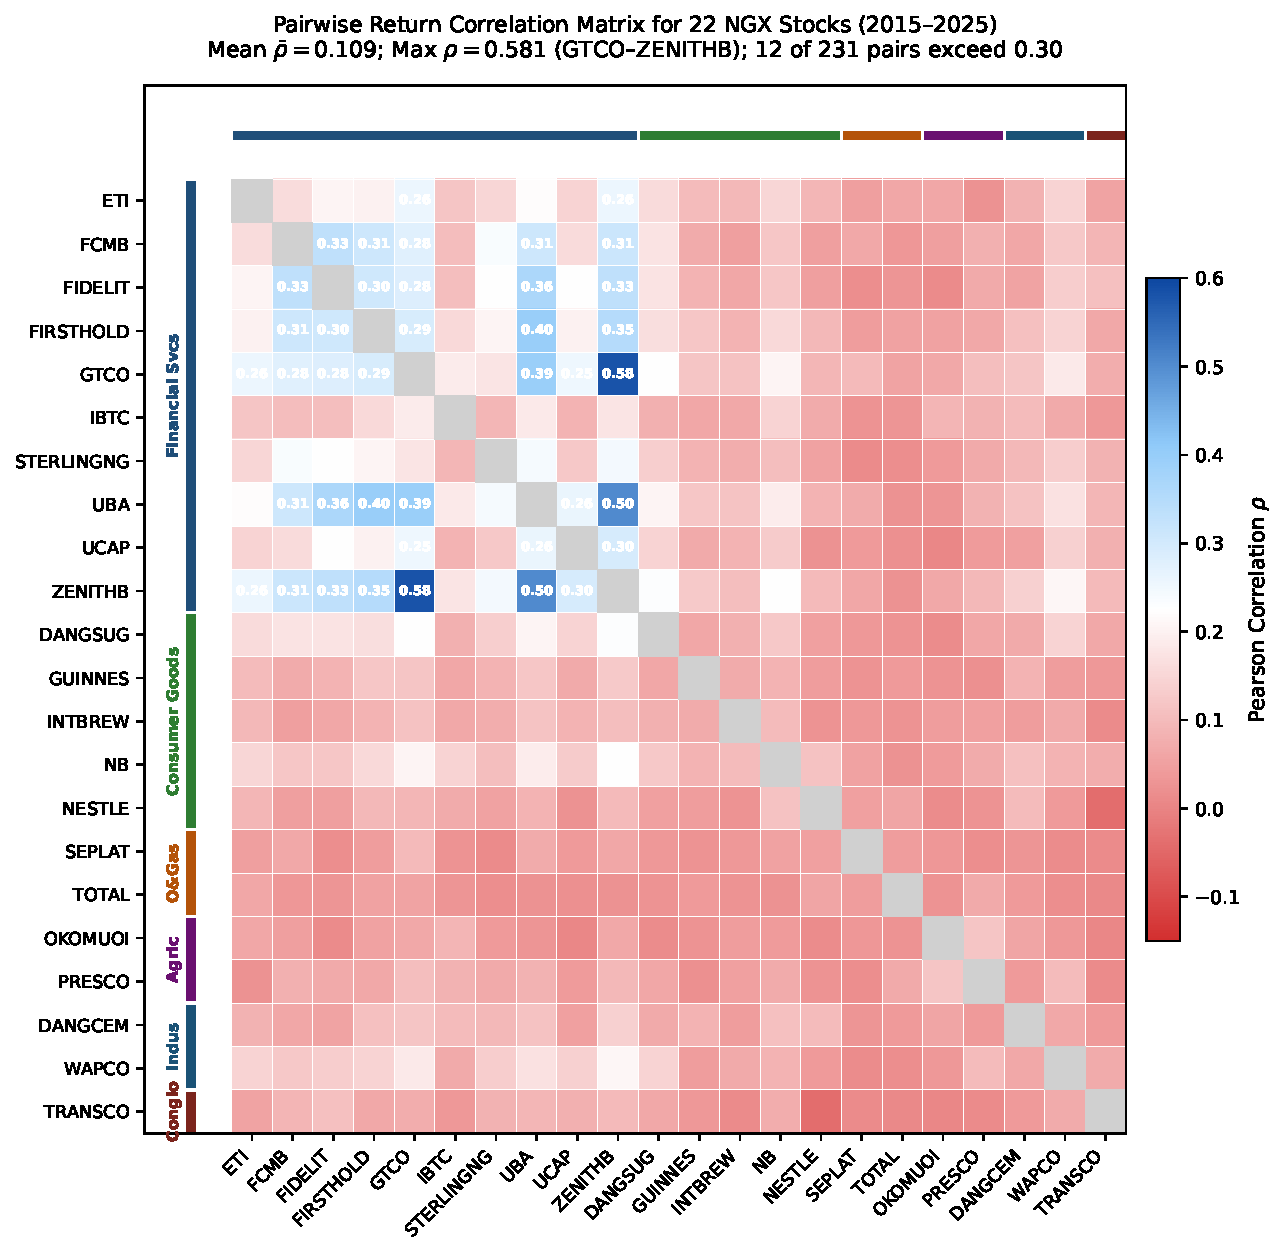
\includegraphics[width=\linewidth]{fig1_correlation_heatmap.pdf}\caption{Pairwise return correlation matrix for the 22-stock
			\ngx\ universe (2015--2025), sorted by sector. Values
			annotated for pairs exceeding $\rho = 0.25$. The
			banking-sector cluster (top-left block) is the dominant
			structural feature; FCMB, FIDELIT, FIRSTHOLD, GTCO, UBA,
			and ZENITHB show correlations from 0.31 to 0.58 while the
			remainder of the matrix is largely sparse.}
		\label{fig:corr_heatmap}
		\vspace{-20pt}
	\end{figure}
	\newpage
	% ============================================================
	\section{Market Efficiency}
	\label{sec:efficiency}
	
	ADF tests on price levels yield $p$-values from 0.465 (NB) to 1.000 (OKOMUOI): every stock fails to reject the unit root null at any conventional significance level, confirming $I(1)$ prices consistent with weak-form efficiency in levels. Returns, however, are not entirely serially independent. The cross-sectional mean lag-1 autocorrelation is $+0.032$ (standard deviation 0.083), and eight stocks exceed $|\hat{\rho}_1| > 0.10$:
	
	\begin{center}
		\small
		\begin{tabular}{lcc}
			\toprule
			\textbf{Stock} & $\hat{\rho}_1$ & \textbf{Direction}\\
			\midrule
			ZENITHB    & $+0.158$ & Momentum\\
			FIRSTHOLD  & $+0.156$ & Momentum\\
			GUINNES    & $+0.150$ & Momentum\\
			WAPCO      & $-0.154$ & Reversal\\
			DANGSUG    & $+0.108$ & Momentum\\
			NB         & $+0.107$ & Momentum\\
			GTCO       & $+0.101$ & Momentum\\
			SEPLAT     & $+0.100$ & Momentum\\
			\bottomrule
		\end{tabular}
	\end{center}
	
	Seven of the eight show positive momentum autocorrelation. The
	exception is WAPCO ($-0.154$), whose reversal pattern is consistent with bid-ask bounce or microstructure noise in a stock whose median/mean volume ratio of 0.041 signals highly sporadic trading. The autocorrelations are modest in magnitude but their presence across 8 of 22 stocks is consistent with the partial predictability documented for other thin African equity markets \citep{ferrouhi2021calendar}, and leaves open a channel for short-horizon linear signal. For the GNN pre-selection module this means return history features lagged returns and rolling momentum signals belong in the node-level feature set alongside technical indicators, not just graph-level inter-stock dependencies. The seven momentum stocks are natural candidates for trend-following inputs; WAPCO's reversal pattern warrants a mean-reversion feature specifically calibrated to its volume episodicity.
	
	% ============================================================
	\section{International Benchmark Comparison}
	\label{sec:comparison}
	\vspace{-20pt}
	\begin{table}[ht]
		\centering
		\caption{International benchmark comparison over 2015--2025.	Returns and volatility are annualised; Sharpe ratio uses a 0\% risk-free rate for cross-market comparability.	All \ngx\ figures are in nominal Naira terms.$^*$}
		\label{tab:comparison}
		\small
		\begin{tabular}{lrrrrr}
			\toprule
			\textbf{Market} & \textbf{Ret (\%)} & \textbf{Vol (\%)} &
			\textbf{Sharpe} & \textbf{Skew} & \textbf{Kurt}\\
			\midrule
			NGX (Composite)$^*$ & 26.5 & 19.0 & 1.40 & $+1.62$ & 18.65\\
			S\&P 500            & 12.6 & 17.9 & 0.71 & $-0.36$ & 15.10\\
			MSCI EM             &  7.5 & 20.4 & 0.37 & $-0.50$ &  7.90\\
			\bottomrule
		\end{tabular}
		\begin{minipage}{0.96\linewidth}
			\small\vspace{4pt}
			$^*$\textit{Naira devaluation caveat}: The Naira depreciated	sharply against the US Dollar during 2023--2024 following	removal of the CBN exchange rate peg, falling from approximately \$1 = \textsterling{}480 to	\textsterling{}1,500 at peak dislocation. Nominal Naira-denominated returns are inflated relative to USD-equivalent figures for this sub-period; the Sharpe ratio
			advantage would be substantially reduced on a
			currency-adjusted basis. The composite result nonetheless	characterises the return environment faced by a domestic Nigerian investor on its own terms.
		\end{minipage}
	\end{table}
	
	The \ngx\ composite delivers the highest annualised return (26.5\%)	and Sharpe ratio (1.40) of the three indices nearly twice the \spidx\ (0.71) and almost four times \msciem\ (0.37) at comparable volatility (19.0\% versus 17.9\% and 20.4\%). It also exhibits positive skewness (+1.62) where both benchmarks are negatively skewed, a distributional asymmetry that favours the
	market on tail-risk grounds. Composite kurtosis (18.65) remains	above both benchmarks despite index-level diversification, which reflects the fat-tailed individual stock distributions documented in Section~\ref{sec:dist}.
	
	Two caveats apply. The composite Sharpe ratio of 1.40 partly reflects diversification mechanics: mean stock-level volatility is 43.3\% against an index volatility of 19.0\%, and individual Sharpe	ratios range from 0.08 (NB) to 1.18 (PRESCO) with a cross-sectional
	mean of 0.57. Additionally, the 2023--2024 Naira devaluation inflated terminal nominal returns materially; a rolling Sharpe analysis reserved for the full research paper is needed to establish whether the composite advantage holds consistently across the decade or concentrates in the post-devaluation recovery window.
	
	% ==========================================================
	\section{Implications for ML Portfolio Design}
	\label{sec:implications}
	
	The five findings map to five design requirements for the two-stage GNN--RL framework \citep{huang2024}, summarised here in consolidated form.
	
	\textbf{Downside-sensitive reward functions.} Median excess kurtosis of 4.79 and CVaR--VaR spreads exceeding 200 bps universally rule out Gaussian-based optimisation objectives. The RL agent's reward function
	\citep{liang2024portfolio, jiang2024drl} must penalise drawdown and CVaR rather than symmetric variance.
	
	\textbf{Adaptive volatility features.} With median GARCH persistence	at 0.912, static covariance estimates are systematically biased during regime transitions. The RL state space must include rolling realised variance and GARCH-implied conditional variance, consistent with the
	advantage that adaptive RL agents hold over static optimisers in non-stationary frontier environments \citep{ngo2023frontier}.
	
	\textbf{Constrained rebalancing frequency.} Nine stocks with median/mean volume below 0.30 cannot absorb institutional block trades daily. The action space must target weekly or monthly intervals with transaction cost penalties calibrated to \ngx\ market impact rather
	than the near-zero friction embedded in \spidx-trained models.
	
	\textbf{GNN attention over raw correlation.} With 5.2\% of pairs exceeding $\rho = 0.30$, the market offers no single-block systematic structure for a correlation-only model to exploit. The GNN attention mechanism \citep{wu2021comprehensive, sun2024graphsage} learns
	inter-stock relevance weights from the data, making it well-suited to extract signal from a sparse matrix. The banking cluster serves as a ground-truth validation target for the learned attention weights.
	
	\textbf{Hard exclusion filters for structural outliers.} TRANSCO	(persistence 1.000, kurtosis 968.4) and UCAP (kurtosis 64.4) cannot	be modelled by any standard distribution and will destabilise training if retained. Volatility persistence thresholds and kurtosis screens
	must act as hard gates before any model sees the data.
	
	% ==========================================================
	\section{Conclusion}
	\label{sec:conclusion}
	
	The Nigerian Stock Exchange has five structural properties that collectively disqualify generic ML portfolio models trained on	developed-market data: universal non-normality with positive skewness and fat tails; high and persistent conditional volatility (mean 43.3\% annualised, median GARCH persistence 0.912); liquidity risk that	operates through volume episodicity rather than zero-volume absence; a sparse correlation matrix ($\bar{\rho} = 0.109$) with a single	dominant banking-sector cluster; and risk-adjusted composite returns	that compare favourably with global benchmarks on nominal terms, subject to the Naira devaluation caveat of Section~\ref{sec:comparison}. Two stocks; TRANSCO and UCAP, are structural outliers that require hard exclusion filters before any model is trained.
	
	These are not incidental data characteristics. Each one determines whether a specific modelling choice is valid or will fail out-of-sample. The GNN--RL framework being developed as the next stage of this research programme is designed with each constraint in mind: downside-sensitive reward functions, adaptive volatility state features, weekly-to-monthly rebalancing constraints, attention-based graph construction calibrated to the sparse correlation structure, and statistical screening gates at the data ingestion layer. This characterisation is the empirical contract that the model must honour.
	
	Three extensions are planned: asymmetric GARCH specifications (EGARCH, GJR-GARCH) to test for leverage effects given the prevalent positive skewness; dynamic conditional correlation estimation for time-varying covariance inputs; and cross-market validation on the Johannesburg Stock Exchange to assess how much
	of what we find here is Nigeria-specific and how much generalises across the continent.
	
	% ==========================================================
	\section*{Data Availability Statement}
	\label{sec:data_availability}
	
	The daily OHLCV data for the 22 \ngx\ constituent stocks analysed in this study were obtained from the Nigerian Stock Exchange (NGX) official data portal (\url{https://ngxgroup.com}) and cross-validated
	against Investing.com (\url{https://www.investing.com}). Macroeconomic series (exchange rates, monetary policy rates, consumer price index) were sourced from the Central Bank of Nigeria	(\url{https://www.cbn.gov.ng}) and the Nigerian Bureau of Statistics (\url{https://www.nigerianstat.gov.ng}). All source data are publicly accessible through the cited portals under their respective terms of use.
	
	The cleaned dataset, computed features, and analysis code (Python, using \texttt{pandas}, \texttt{arch}, \texttt{scipy}, and	\texttt{statsmodels}) used to produce all tables and statistics reported in this paper are available in the supplementary materials submitted alongside this manuscript. A permanent repository link
	will be provided upon acceptance of the full doctoral research paper of which this study forms the empirical foundation.
	
	% -------------------------------------------------------
	% Acknowledgement
	% -------------------------------------------------------
	\begin{acks}
		The authors thank the supervisory team at the Centre for Cyberspace Studies, Nasarawa State University, Keffi, for guidance throughout this work. The authors declare no competing financial interests in any \ngx-listed equity security. No external funding was received for this work at the time of submission.
	\end{acks}
	
	\vskip 0.2in
	\bibliography{references}
	
\end{document}